\documentclass{article}

    \title{Document title}
    \date{Date}
    \author{Anurag Kapur [Anurag.Kapur@kellogg.ox.ac.uk]}

    \usepackage{afterpage}
    \newcommand\blankpage{%
        \null
        \thispagestyle{empty}%
        \addtocounter{page}{-1}%
        \newpage}

    \usepackage[subpreambles=true]{standalone}
    \usepackage{tikz}
    \usepackage{tikz-qtree}
    \usetikzlibrary{trees}

\begin{document}

    \maketitle
    \pagenumbering{gobble}

    \afterpage{\blankpage}

    \newpage
    \pagenumbering{arabic}
    \tableofcontents

    \newpage
    \section{Section 1}
    \subsection{Sub-section 1}

    \newpage
    \section{Section 2}
    \subsection{Sub-section 2}

    \begin{figure}[!htb]
      \subsubsection{Sub section}
      \centering
      \includestandalone[mode=buildnew]{trees}
      \caption{interesting results}
    \end{figure}

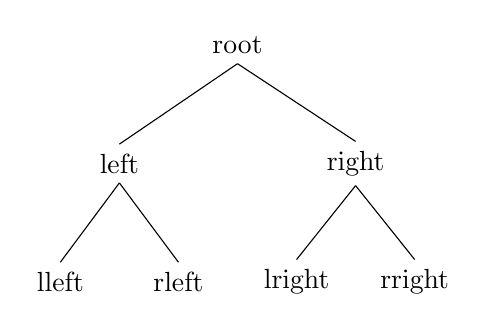
\begin{tikzpicture}[level distance=1.5cm,
  level 1/.style={sibling distance=3cm},
  level 2/.style={sibling distance=1.5cm}]
  \node {root}
    child {node {left}
      child {node {lleft}}
      child {node {rleft}}
    }
    child {node {right}
    child {node {lright}}
      child {node {rright}}
    };
\end{tikzpicture}

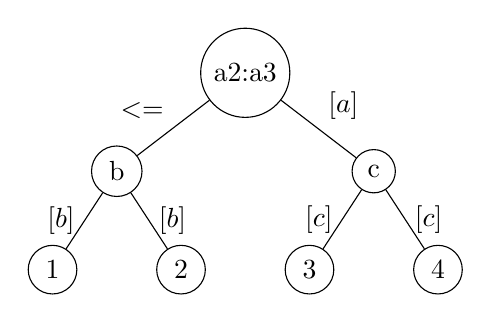
\begin{tikzpicture}[every tree node/.style={draw,circle},
   level distance=1.25cm,sibling distance=1cm,
   edge from parent path={(\tikzparentnode) -- (\tikzchildnode)}]
\Tree
[.a2:a3
    \edge node[auto=right] {$<=$};
    [.b
       \edge node[midway,left] {$[b]$};
       [.1 ]
       \edge node[midway,right] {$[b]$};
       [.2 ]
        ]
    \edge node[auto=left] {$[a]$};
    [.c
        \edge node[midway,left] {$[c]$};
        [.3 ]
        \edge node[midway,right] {$[c]$};
        [.4 ]
        ]
]
\end{tikzpicture}

\end{document}